\documentclass[a4paper,12pt]{article} % тип документа
\usepackage[margin=1in]{geometry} % Поля

%  Русский язык
\usepackage[warn]{mathtext}
\usepackage[T2A]{fontenc}			% кодировка
\usepackage[utf8]{inputenc}			% кодировка исходного текста
\usepackage[english,russian]{babel}	% локализация и переносы
% Математика
\usepackage{amsmath,amsfonts,amssymb,amsthm,mathtools} 
\usepackage{wasysym}
%%%
\usepackage{graphicx}

\usepackage{tabularx}

\usepackage{gensymb} % знак градуса
\usepackage{enumitem} % изменить список enumerate
\usepackage{placeins} % \FloatBarrier

\renewcommand{\thesection}{\Roman{section}} 
\renewcommand{\thesubsection}{\roman{subsection}}


\begin{document}

\newcolumntype{Y}{>{\centering\arraybackslash}X} %new tabularx


%титул
\hrule 	
\medskip
\begin{raggedright}
{\large \textbf{Отчёт по работе 6.11.5}}
\\
\medskip
{\Large Туннелирование в полупроводниках} 
\\
\medskip
{\large Карташов Констанин Б04-005}
\medskip
\hrule
\medskip
\end{raggedright}


\paragraph{Цель работы:} 
Исследуется принцип действия туннельного диода, измеряются его вольт-амперная характеристика и основные параметры.

\medskip\hrule\medskip

\section{Теоретическая часть}

\paragraph{}
	Туннельный диод или диод Эсаки (изобретён Лео Эсаки в 1957 году) -- полупроводниковый диод на основе вырожденного полупроводника, на вольт-амперной характеристике которого при приложении напряжения в прямом направлении имеется участок с отрицательным дифференциальным сопротивлением, обусловленный туннельным эффектом. Туннельный диод представляет собой p-n-переход, обе области в котором имеют предельно сильное, до вырождения, легирование -- концентрации доноров $n_n$ в n-области и акцепторов $n_p$ в p-области могут превышать $10^{19}$ см$^{-3}$.

\paragraph{}
	Расстояния от уровня Ферми до краев зон:
	\begin{equation}
		\begin{gathered}
			\xi = \mu_n - E_c,\\
			\eta = \mu_p - E_v.
		\end{gathered}
	\end{equation}

	 При достижении $U_v$ ток через диод минимален, что соответствует совпадению границ зоны проводимости $E_c$ и валентной зоны $E_v$. Откуда можно оценить положение уровней Ферми:
	 
	\begin{equation}
		eU_v \approx \xi + \eta \approx 2\xi \approx 2\eta.
		\label{e:fermi}
	\end{equation}

	Напряжению $U_p$ соответствует пик тока, при котором смещение энергетических зон должно быть одинаково. Это даёт возможность определить энергетический промежуток $E_{n \max}$ между уровнем Ферми и максимум плотности распределения электронов $n_{\max}(E)$, отсчитываемый от границы зоны проводимости:
	\begin{equation}
		eU_p \approx \xi - E_{n\max}.
		\label{e:energ}
	\end{equation}

\medskip\hrule\medskip

\section{Экспериментальная часть}

\subsection{Экспериментальная установка}

\paragraph{}
	Для измерения основных параметров туннельного диода используются три различные схемы.
	
	При снятии вольт-амперной характеристики и определении параметров туннельного диода (рис. \ref{fig:setup_vac}) ток измеряется амперметром, включенным последовательно с туннельным диодом, а напряжение на диоде измеряется вольтметром. Регулирование тока через диод производится переменным сопротивлением $R$. Ключи $K_1$ и $K_2$ используются при уточнении основных параметров диода.

\begin{figure}[h]
\centering
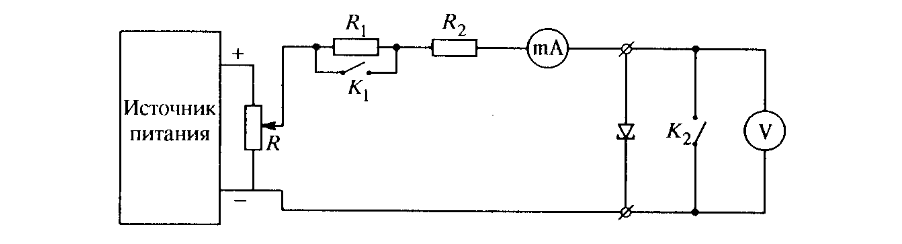
\includegraphics[width=\textwidth]{setup_vac.png}
\caption{Принципиальная схема измерения параметров вольт-амперной характеристики туннельного диода}
\label{fig:setup_vac}
\end{figure}

\paragraph{}
	Быстрее и нагляднее, но с меньшей точностью можно измерить характеристику диода с помощью осциллографа и мостовой схемы, изображенной на рис. \ref{fig:setup_osc}. На вход <<Y>> осциллографа подаётся напряжение, пропорциональное току, протекающему через диод, а на вход  <<X>>  -- падение напряжения на диоде. Ток протекающий через диод можно определить по формуле:
	
	\begin{equation}
	I_D = U_D \frac{R_1 + 2(R_2 + R_3)}{(R_1 + 2 R_2)R_3},
	\label{e:res}
	\end{equation}
	
	\noindent где $R_1$, $R_2$ и $R_3$ -- сопротивления соответствующих резисторов в плечах моста. Напряжение $U_D$ определяется с помощью осциллографа. 

\begin{figure}[h]
\centering
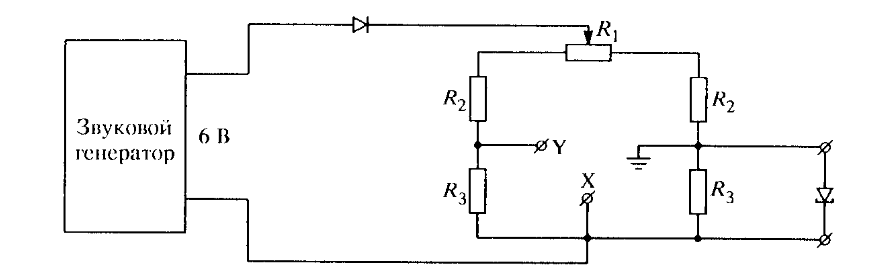
\includegraphics[width=\textwidth]{setup_osc.png}
\caption{Принципиальная схема наблюдения вольт-амперной характеристики туннельного диода с помощью осциллографа}
\label{fig:setup_osc}
\end{figure}


\paragraph{}
	Генератор электромагнитных колебаний на туннельном диоде собран по схеме с параллельным контуром (рис. \ref{fig:setup_gen}). Резистор и конденсатор служат для развязки источника питания и генератора по переменному напряжению. Резистор служит для выведения рабочей точки туннельного диода на нужную ветвь вольт-амперной характеристики.


\begin{figure}[h]
\centering
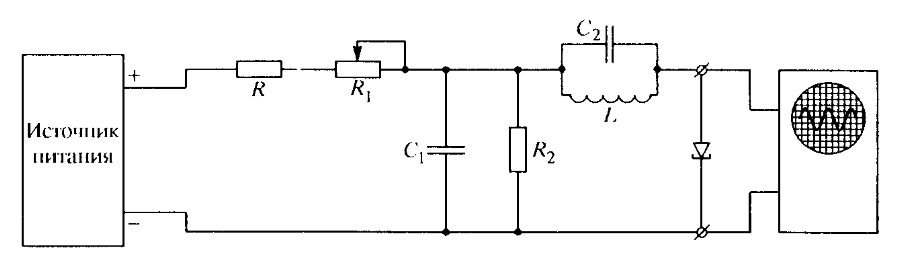
\includegraphics[width=\textwidth]{setup_gen.png}
\caption{Принципиальная схема генератора на туннельном диоде}
\label{fig:setup_gen}
\end{figure}

\subsection{Наблюдение вольт-амперной характеристики туннельного диода с помощью осциллографа}

\paragraph{}
	Воспользуемся схемой изображённой на рис. \ref{fig:setup_osc}. На нашей схеме $R_1 = 680$ Ом, $R_2 = 100$ Ом, $R_3 = 120$. Поэтому формула \eqref{e:res} принимает вид $I_D = U_D / R$, где $R = 94.3$ Ом.
	
	Получим на осциллографе изображение вольт-амперной характеристики при масштабных коэффициентах $\alpha_X = 50$ мВ/дел, $\alpha_Y = 100$ мВ/дел (рис \ref{fig:osc}).
	
	\begin{figure}[h]
	\centering
	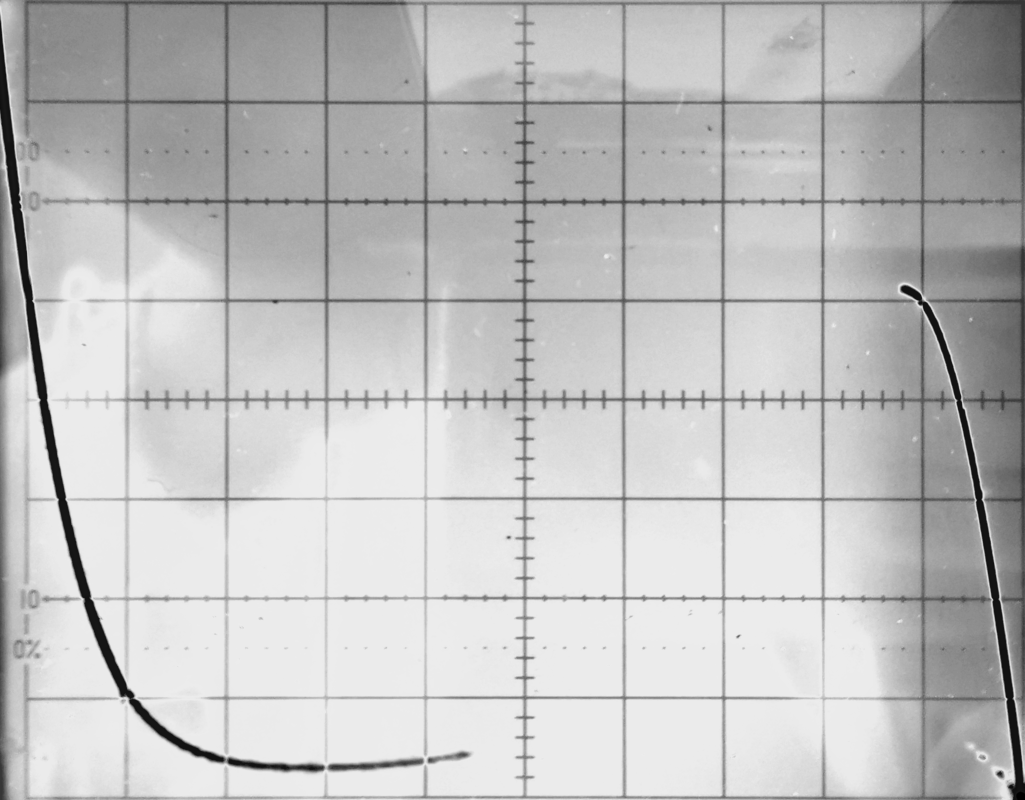
\includegraphics[width=0.5\textwidth]{vac_osc.png}
	\caption{Вольт-амперная характеристика, полученная на осциллографе}
	\label{fig:osc}
	\end{figure}
	
	По полученной вольт-амперной характеристике определим значения $U_p, U_v, U_f$ и $I_p, I_v$, погрешность оценим по ширине кривой на экране осциллографа:
	
\[
U_p = 1.2 \pm 0.1 \text{ дел} = 60 \pm 5 \text{ мВ},
\]\[
U_v = 7.2 \pm 0.2 \text{ дел} = 360 \pm 10 \text{ мВ},
\]\[
U_f = 10 \pm 0.1 \text{ дел} = 500 \pm 5 \text{ мВ},
\]\[
U_{I_p} = 5.1 \pm 0.1 \text{ дел} = 510 \pm 10  \text{ мВ} \; \Rightarrow \; I_p = U_{I_p} / R = 5.4 \pm 0.1 \text{ мА},
\]\[
U_{I_v} = 0.3 \pm 0.1 \text{ дел} = 30 \pm 10  \text{ мВ} \; \Rightarrow \; I_v = U_{I_v} / R = 0.3 \pm 0.1 \text{ мА}.
\]
	
\subsection{Получение статической характеристики туннельного диода}

\paragraph{}  
	Воспользуемся схемой изображённой на рис. \ref{fig:setup_vac}. Меняя значения переменного сопротивления $R$ снимем вольт-амперную характеристику диода. Измеренные данные приведены в таблице \ref{tab:vac}. 

\begin{table}[h]
\centering
\begin{tabular}{|c|c|c|c|c|c|c|c|}
\cline{1-2} \cline{4-5} \cline{7-8}
$U$, мВ & $I$, мА &  & $U$, мВ & $I$, мА &  & $U$, мВ & $I$, мА \\ \cline{1-2} \cline{4-5} \cline{7-8} 
1       & 0.004   &  & 226.2   & 2.024   &  & 408.7   & 0.676   \\ \cline{1-2} \cline{4-5} \cline{7-8} 
5.3     & 0.958   &  & 333.7   & 0.91    &  & 419.5   & 0.784   \\ \cline{1-2} \cline{4-5} \cline{7-8} 
10.4    & 1.8     &  & 345.5   & 0.828   &  & 445.4   & 1.314   \\ \cline{1-2} \cline{4-5} \cline{7-8} 
15.6    & 2.539   &  & 353.4   & 0.785   &  & 459.7   & 1.778   \\ \cline{1-2} \cline{4-5} \cline{7-8} 
21.8    & 2.262   &  & 362     & 0.739   &  & 460.7   & 1.814   \\ \cline{1-2} \cline{4-5} \cline{7-8} 
28.2    & 3.825   &  & 386     & 0.524   &  & 464.2   & 1.855   \\ \cline{1-2} \cline{4-5} \cline{7-8} 
30.3    & 3.98    &  & 391.1   & 0.538   &  & 486.3   & 3.69    \\ \cline{1-2} \cline{4-5} \cline{7-8} 
33      & 4.138   &  & 392.5   & 0.546   &  & 493.3   & 4.578   \\ \cline{1-2} \cline{4-5} \cline{7-8} 
41.6    & 4.15    &  & 397.7   & 0.582   &  & 494.6   & 4.748   \\ \cline{1-2} \cline{4-5} \cline{7-8} 
50.2    & 4.15    &  & 402     & 0.609   &  & ---     & ---     \\ \cline{1-2} \cline{4-5} \cline{7-8} 
\end{tabular}
\caption{Снятые точки для вольт-амперной характеристики}
\label{tab:vac}
\end{table}

\paragraph{}
	По данным из таблицы \ref{tab:vac} построим график вольт-амперной характеристики (рис. \ref{fig:plot}). Теоретическая погрешность значений полученных статическим методом ограничена погрешностью измерительных приборов, однако на практике измерения вблизи точек $p$ и $v$ становятся неточными из-за близости к неустойчивым участкам вольт-амперной характеристики, погрешность внесённую неустойчивостью сложно оценить. Оценим погрешность как половину разности значения между ближайшими точками в измерении, тогда $\Delta U \sim 1$ мВ, $\Delta I \sim 0.01$ мА. Полученные значения:
	
	\[ U_p = 50 \text{ мВ}, \; I_p = 4.15 \text{ мА}, \; U_v = 386 \text{ мВ}, \; I_v = 0.52 \text{ мА}, \; U_f = 490 \text{ мВ} \]
	
	
\begin{figure}[h]
\centering
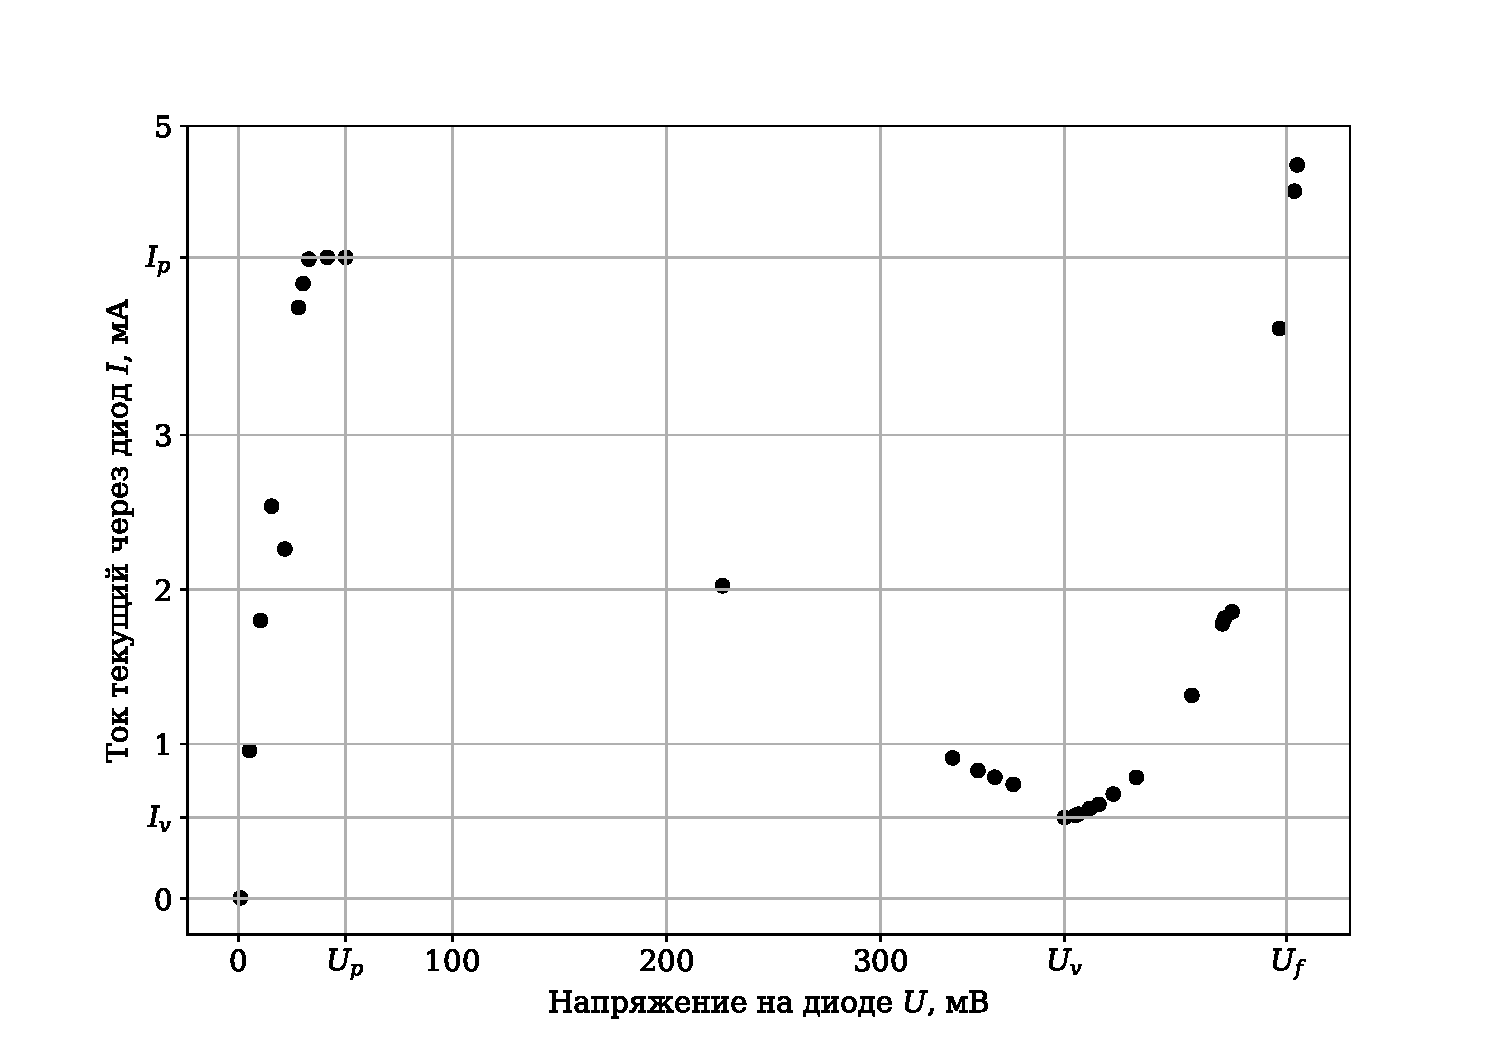
\includegraphics[width=\textwidth]{plot.pdf}
\caption{График вольт-амперной характеристики снятой статическим методом}
\label{fig:plot}
\end{figure}

\paragraph{} Оценим по измеренным данным и формулам \eqref{e:fermi} и \eqref{e:energ} энергию Ферми и энергию соответствующую максимальной плотности распределения электронов:

\[
\mu_n \approx \mu_p = \mu = \frac{eU_v}{2}, \; \Delta \mu = \frac{e \Delta U_v}{3},
\]\[ 
E_{n_{\max}} = \mu - eU_p, \; \Delta E_{n_{\max}} = \sqrt{(\Delta \mu)^2 + (e \Delta U_p)^2} = e \sqrt{(\Delta U_p)^2 + \left(\frac{\Delta U_v}{2}\right)^2}
\]
	
\noindent Результаты вычисления приведены в сводной таблице (табл. \ref{tab:results}). 
	
\subsection{Изучение генератора на основе туннельного диода}

\paragraph{}
	Воспользуемся схемой изображённой на рисунке \ref{fig:setup_gen}. Получим на осциллографе изображение колебаний (рис. \ref{fig:generation}). Частота колебаний примерно равна $f \approx 180$ кГц, при изменении сопротивления видимых изменений частоты колебаний и формы волны не происходило, при этом амплитуда колебаний менялась в пределе от $0.5$ до $0.4$ В.

\begin{figure}[h]
\centering
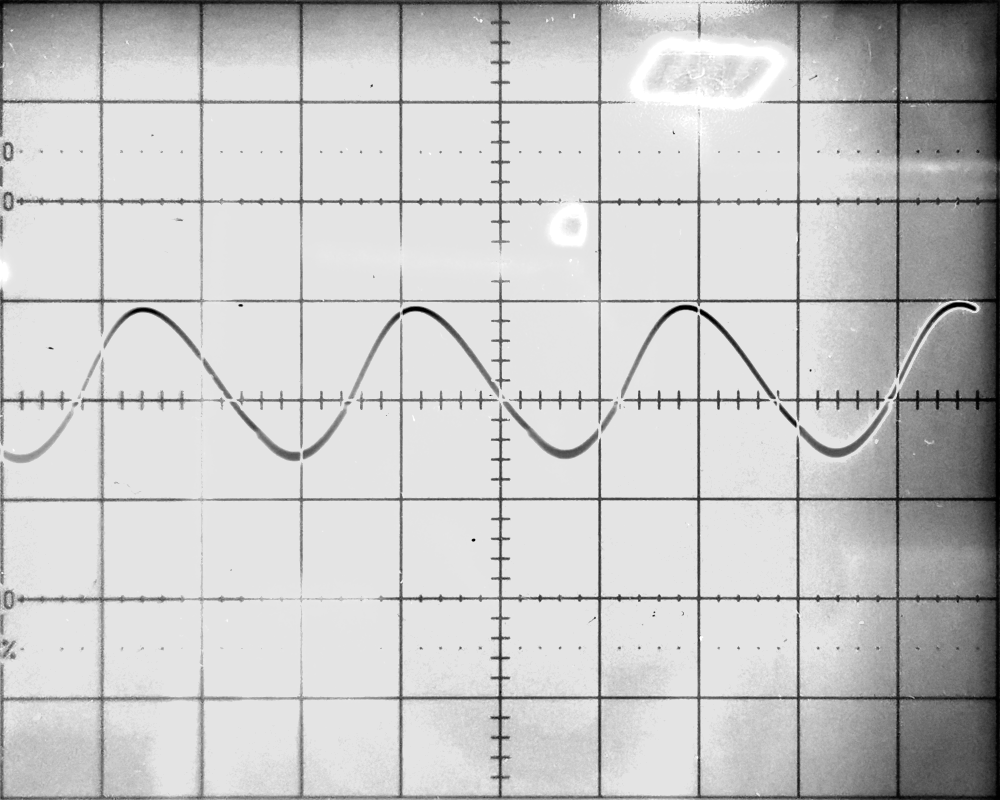
\includegraphics[width=0.5\textwidth]{generation.png}
\caption{Изображение колебаний полученное на осциллографе}
\label{fig:generation}
\end{figure}

\medskip\hrule\medskip

\section{Выводы}

\begin{enumerate}
\item Получили вольт-амперную характеристику туннельного диода на осциллографе. Полученное изображение соответствует теоретическим ожиданиям.
\item Получили вольт-амперную характеристику туннельного диода статическим методом. Полученная зависимость согласовывалась с полученной на осциллографе.
\item По измеренным вольт-амперным характеристикам определили характеристики туннельного диода приведённые в таблице \ref{tab:results}.

\begin{table}[h]
\centering
\small
\begin{tabular}{|l|l|l|l|l|l|l|l|}
\hline
величина & $U_p$, мВ  & $U_v$, мВ    & $U_f$, мВ   & $I_p$, мА       & $I_v$, мА       & $\mu$, мэВ  & $E_{n_{\max}}$, мэВ \\ \hline
динам.   & $60 \pm 5$ & $360 \pm 10$ & $500 \pm 5$ & $5.4 \pm 0.1$   & $0.3 \pm 0.1$   & $180 \pm 5$ & $120 \pm 7$         \\ \hline
стат.    & $50 \pm 1$ & $386 \pm 1$  & $490 \pm 1$ & $4.15 \pm 0.01$ & $0.52 \pm 0.01$ & $193 \pm 1$ & $143 \pm 1$         \\ \hline
\end{tabular}
\caption{Сводная таблица}
\label{tab:results}
\end{table}

\item Изучили сигнал создаваемый генератором на основе туннельного диода.
\end{enumerate}



\medskip\hrule\medskip

\end{document}
